\Chapter{Étude de plasmas magnétisés}
\chaptermark{Étude de plasmas magnétisés}
\begin{refsection}

	\section{Plasma de bord des tokamaks}
		 
	\section{PEGASES, la barrière magnétique}
		\subsection{Comparaison expérimentale}
			
			\subsubsection{Variation de l'intensité du champ magnétique}
			\subsubsection{Variation de l'intensité du champ magnétique}
\begin{figure}[htbp]
\centering
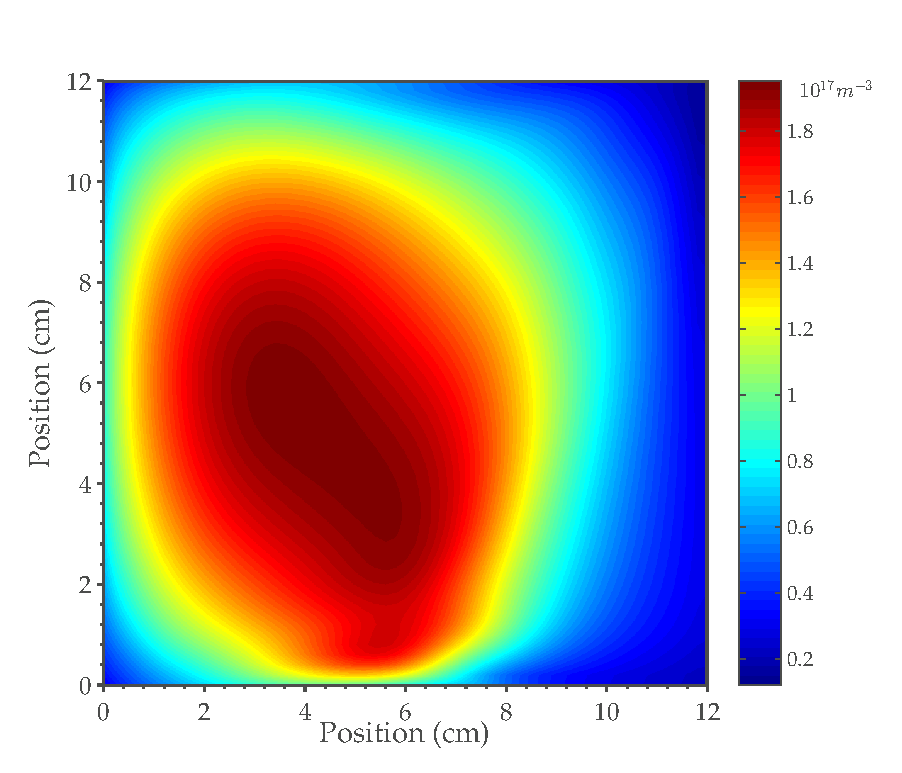
\includegraphics[width=5.5cm]{figures/pegasescarteDensite.eps}
{\caption{Carte de densité dans le propulseur.} \label{4-pegasesDensite}}
\end{figure}
	
	\section{CYBELE Colonne de plasma magnétisé}
	\begin{figure}[htbp]
	\includegraphics[width=0.9\textwidth]{figures/pegasesCarteCourant.eps}{
	\caption{Carte de courants dans le propulseur.} \label{4-pegasesCourants}}
\end{figure}
		

%\bibliographystyle{apalike}
%\bibliography{biblio}
\end{refsection}
